% strumenti per la pubblicazione
% strumenti per l'analisi (TXM, altri)
% slides James Cummings 
% customizzazione TEI vedere capitoli 22 e 23 delle guidelines

% DOM, Javascript XML, XSL
% capitolo 7 testo e automa di ciotti
% SLIDE Chiara sui fogli di stile
% Capitolo DOM professional Web Dev e XML processing
%

\documentclass{beamer}
    
    %    \usepackage[english]{babel}
        %\usepackage[latin1]{inputenc}
        %\usepackage[T1]{fontenc}
    
    \mode<presentation>{
      \setbeamertemplate{background canvas}[vertical shading]
      \usetheme{Berkeley}
      \useoutertheme{himinfolines}
    }
      
    \usepackage{ucs}
    \usepackage[utf8]{inputenc}
    \usepackage[english,polutonikogreek,italian,UKenglish,british]{babel}
    \usepackage{graphicx}
    \usepackage{colortbl}
    \usepackage{multicol}
    \usepackage{ulem}
    \usepackage{verbatim}
    \usepackage{alltt}
    \usepackage{ccicons}
    \usepackage{MnSymbol,wasysym}
    \usepackage{tikzsymbols}
    \usepackage{textcomp}
    \usepackage{xmpincl}
    
    \usepackage{parskip}
    \setcounter{nframes}{68}
    \setcounter{nframe}{1}
    \setbeamercovered{dynamic}
    \newenvironment{grcenv}{\begin{otherlanguage}{greek}}{\end{otherlanguage}}
    \newcommand{\g}[1]{\textgreek{#1}}
    \definecolor{darkgreen}{rgb}{0,0.5,0}
    \definecolor{darkblue}{rgb}{0,0,0.5}
    \definecolor{grey}{rgb}{0.5,0.5,0.5}
    \setcounter{tocdepth}{5}
    
    \makeatletter
    
    \makeatother
    %\includexmp{LicencesAndLicensing}
    
    %frame00 metadata
        \title{Codifica TEI - Personalizzazione e Tematiche avanzate}
        \author[A.M. Del Grosso]{Angelo Mario Del Grosso \\ \tiny\textit{(materiale parzialmente derivato dalle lezioni della Prof. C. Di Pietro))}}
        \institute{\texttt{angelo.delgrosso@ilc.cnr.it} \\\textit{CNR-ILC-LicoLab} \\\url{http://licolab.ilc.cnr.it/}}
        \date{Istituto di Linguistica Computazionale ``A. Zampolli'', \today}
        \AtBeginSection[]{
        \begin{frame}<beamer>
        \addtocounter{nframe}{1}
        \footnotesize
        \frametitle{Progress status}
        \tableofcontents[currentsection,hideothersubsections]
        \end{frame}
        }
    
    \begin{document}
    
    \begin{frame}
        \maketitle
    \end{frame}
    
    \begin{frame}
        \frametitle{Sommario della Lezione}
        \tableofcontents
    \end{frame}
    
    \section{Introduzione}
    
    \begin{frame}
        \frametitle{Visualizzare ed Elaborare documenti XML}
        \addtocounter{nframe}{1}
        
        \begin{center}
            
\includegraphics[width=.7\textwidth]{imgs/tei-r.pdf}
        \end{center}
        %\textit{In parte già disponibili nei moduli TEI di base}

        %  \begin{block}{Perché visualizzare ed elaborare il testo}
        % %     \emph{Per la critica testuale indispensabili i moduli}
        %      \begin{itemize}
        %         \item Controllare la codifica e correggere i refusi
        %         \item Assicurarsi che tutto sia stato trascritto correttamente
        %         \item Mostrare il testo a persone che non conoscono XML-TEI
        %         \item Disporre di una versione del lavoro fruibile
        %         \item Manipolare e analizzare le informazioni codificate
        %     \end{itemize}
        %  \end{block}
        
    \end{frame}
    
    % \begin{frame}
    %     \frametitle{Modularità della TEI}
    %     \addtocounter{nframe}{1}
        
    %    % \begin{center}
    %     % 
\includegraphics[width=.2\textwidth]{../imgs/tei-r.pdf}
    %     % \end{center}
    
    %     \begin{itemize}
            
    %         \item<1-> parleremo del sistema Modulare della TEI
    %             \begin{itemize}
    %                 \item<1-> Moduli
    %                 \item<1-> Classi
    %                 \item<1-> Macro
    %                 \item<1-> Datatype
    %             \end{itemize} 
    %         \item<2-> parleremo degli elementi basilari
    %             \begin{itemize}
    %                 \item<2-> Intestazione TEI (TEIHeader)
    %                 \item<2-> Elementi e attributi presenti in tutti i documenti TEI
    %                 \item<2-> Esempi di codifica
    %             \end{itemize} 
    %     \end{itemize}
        
    % \end{frame}
    
    \section{Personalizzare Schemi TEI}
    
    \begin{frame}
        \frametitle{Modularità e personalizzazione della TEI}
        \addtocounter{nframe}{1}
        
       % \begin{center}
        % 
\includegraphics[width=.2\textwidth]{../imgs/tei-r.pdf}
        % \end{center}
    
        \begin{block}{Vocabolario TEI P5}
            \textbf{Oltre 550 elementi presenti nel vocabolario completo della TEI}
                \begin{itemize}
                    \item Difficilmente serviranno tutti per un singolo progetto
                    \item Probabilmente per un particolare progetto servirà un elemento
                    non previsto
                \end{itemize} 
            \end{block}
    \end{frame}

    \begin{frame}
        \frametitle{Modulatirà e presonalizzazione della TEI}
        \addtocounter{nframe}{1}
        
       % \begin{center}
        % 
\includegraphics[width=.2\textwidth]{../imgs/tei-r.pdf}
        % \end{center}
    
        \begin{block}{Design dello Schema TEI P5}
            
            \textbf{la TEI P5 è progettata per ottimizzare:}
                \begin{itemize}
                    \item aspetti di \textbf{modularità} che consentano agli utenti di selezionare solo le componenti necessarie (moduli).
                    \item aspetti di \textbf{estensiblità} che consentano agli utenti di aggiungere nuovi elementi e attributi
                    \item aspetti di \textbf{riusabilità} che consentano agli utenti di modificare elementi e attributi già esistenti
                \end{itemize} 
        \end{block}
        
    \end{frame}

    \begin{frame}
        \frametitle{Modulatirà e presonalizzazione della TEI}
        \addtocounter{nframe}{1}
        
       % \begin{center}
        % 
\includegraphics[width=.2\textwidth]{../imgs/tei-r.pdf}
        % \end{center}
    
        \begin{block}{Personalizzare lo schema TEI P5}
            
            \textbf{la TEI P5 mette a disposizione}
                \begin{itemize}
                    \item vocabolario XML per la codifica di fenomeni testuali (concetti del testo)
                    \item sistema di moduli e di personalizzazione del vocabolario
                    \item strumenti per la personalizzazione: TEI Roma e ODD
                    \item [] \url{http://www.tei-c.org/Roma/}
                \end{itemize} 
        \end{block}
        
    \end{frame}

    \begin{frame}
        \frametitle{Modulatirà e presonalizzazione della TEI}
        \addtocounter{nframe}{1}

        \begin{block}{alcuni elementi strutturali importanti distinguibili in un libro}
                \begin{itemize}
                    \item Il documento, la pagina del titolo, i capitoli
                    \item Le intestazioni, le sezioni e sotto-sezioni, i paragrafi
                    \item Le citazioni, i discorsi diretti
                    \item Le interruzioni di pagina e di linea
                    \item Le figure, i nomi di persone, i nomi di luoghi
                \end{itemize} 
        \end{block}
        
    \end{frame}


    \begin{frame}
        \frametitle{Modulatirà e presonalizzazione della TEI}
        \addtocounter{nframe}{1}

        \begin{block}{Due possibili strade di personalizzazione}
                \begin{itemize}
                    \item Scegliere una delle personalizzazioni pronte all’uso disponibili sul sito della TEI
                    \item Creare da zero il proprio schema TEI
                \end{itemize} 
        \end{block}
        
    \end{frame}


    \begin{frame}
        \frametitle{Modulatirà e presonalizzazione della TEI}
        \addtocounter{nframe}{1}

        \begin{block}{Scegliere personalizzazione già esistenti}
                \begin{itemize}
                    \item \url{http://www.tei-c.org/Guidelines/Customization/}
                    \item Incentrati su particolari aspetti e caratteristiche del testo
                    \item Da utilizzare così come sono, oppure da sfruttare come punto di
                    partenza per una propria personalizzazione
                \end{itemize} 
        \end{block}
        
    \end{frame}

    \begin{frame}
        \frametitle{Modulatirà e presonalizzazione della TEI}
        \addtocounter{nframe}{1}
        
        \textbf{Utilizzo di customizzazioni già esistenti}

         \begin{center}
            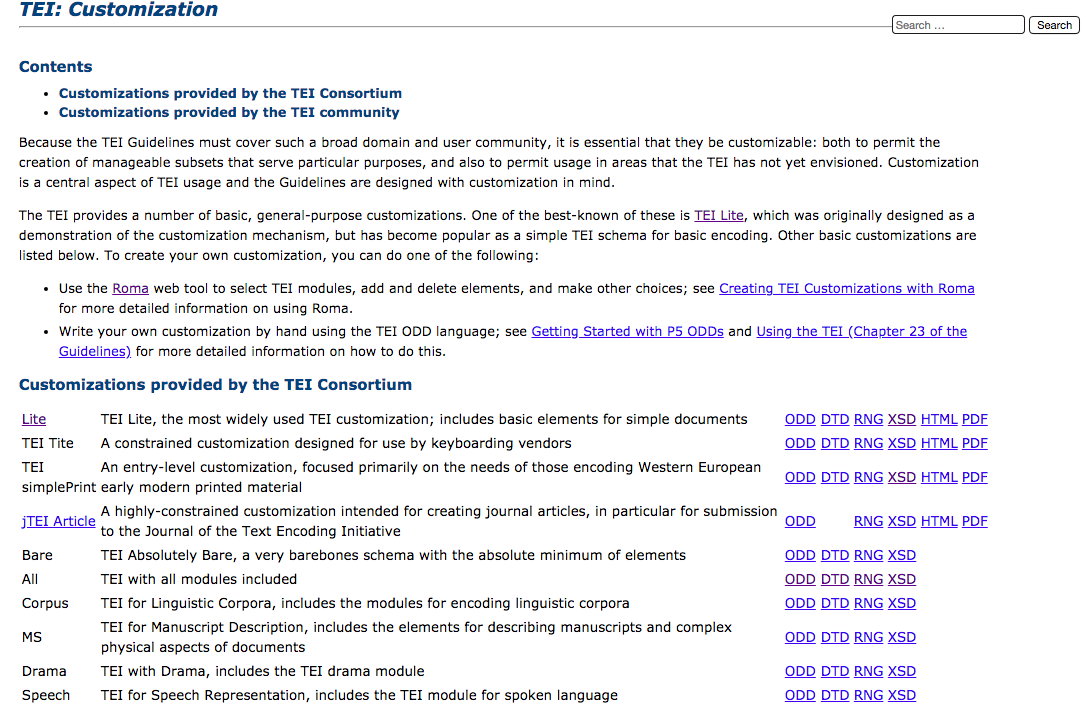
\includegraphics[width=.9\textwidth]{imgs/customization.png}
         \end{center}
       
        
    \end{frame}

    \begin{frame}
        \frametitle{Modulatirà e presonalizzazione della TEI}
        \addtocounter{nframe}{1}

        \begin{block}{Creare da zero il proprio schema TEI}
                \begin{itemize}
                    \item TEI Roma: \url{http://www.tei-c.org/Roma/}
                    \item Selezione e restrizione del modello TEI
                    \item Estensione del modello TEI
                \end{itemize} 
        \end{block}
        
    \end{frame}

    \begin{frame}
        \frametitle{Modulatirà e presonalizzazione della TEI}
        \addtocounter{nframe}{1}
        
        \textbf{Creazione di uno schema con l'applicazione Web Roma}

         \begin{center}
            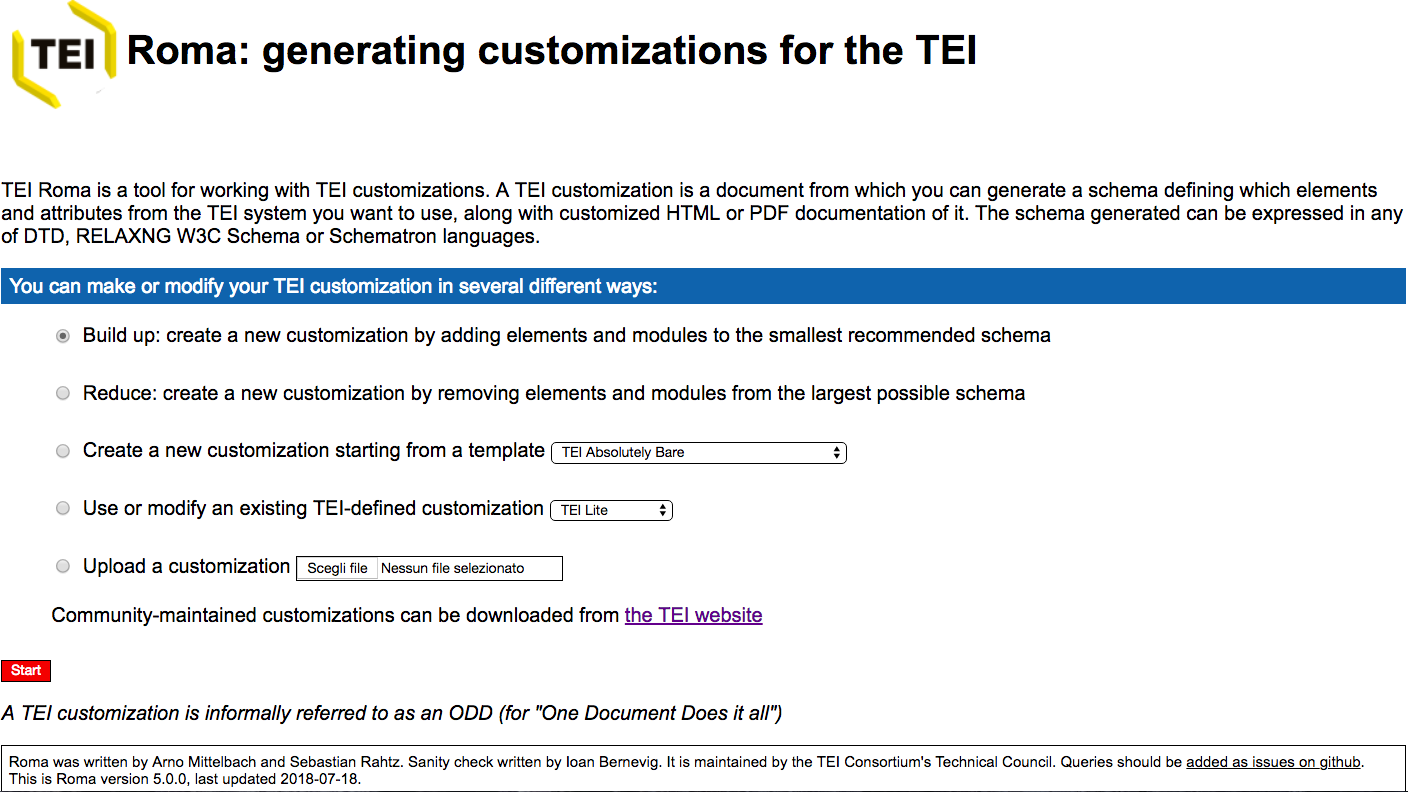
\includegraphics[width=.95\textwidth]{imgs/Roma1.png}
         \end{center}
       
        
    \end{frame}

    \begin{frame}
        \frametitle{Modulatirà e presonalizzazione della TEI}
        \addtocounter{nframe}{1}
        
        \textbf{Passo 1: Inizializzare la personalizzazione}

         \begin{center}
            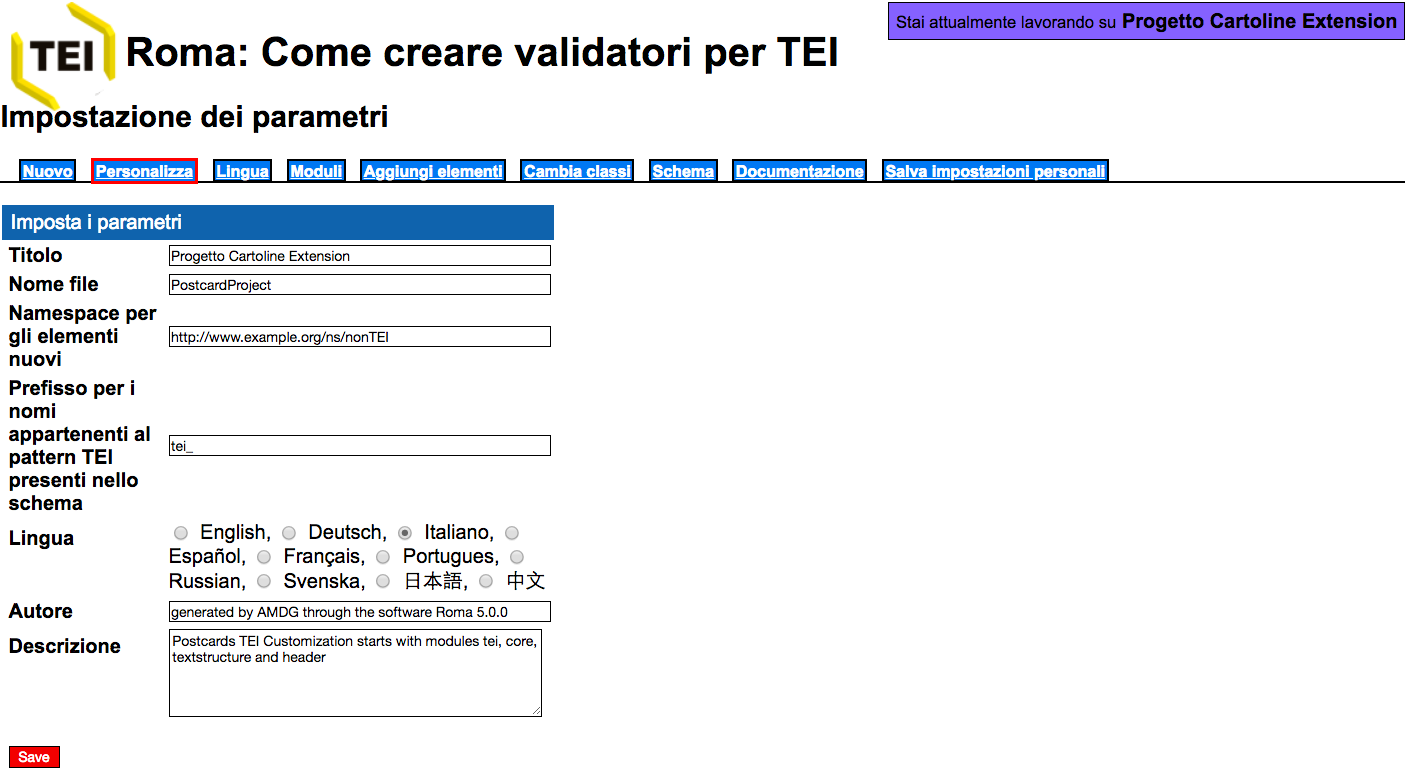
\includegraphics[width=.95\textwidth]{imgs/Roma2.png}
         \end{center}
       
        
    \end{frame}

%     ▪ New → scelta del punto di partenza
% ▪ Customize → personalizzazione metadati
% ▪ Language → lingua schema e documentazione
% ▪ Modules → scelta degli elementi TEI
% ▪ Add Elements → aggiunta elementi
% ▪ Change classes → gestione attributi
% ▪ Schema → generazione schema
% ▪ Documentation → creazione documentazione
% ▪ Save Customization → salvataggio file ODD


\begin{frame}
    \frametitle{Modulatirà e presonalizzazione della TEI}
    \addtocounter{nframe}{1}
    
    \textbf{Passo 2: Selezionare la lingua dello schema}

     \begin{center}
        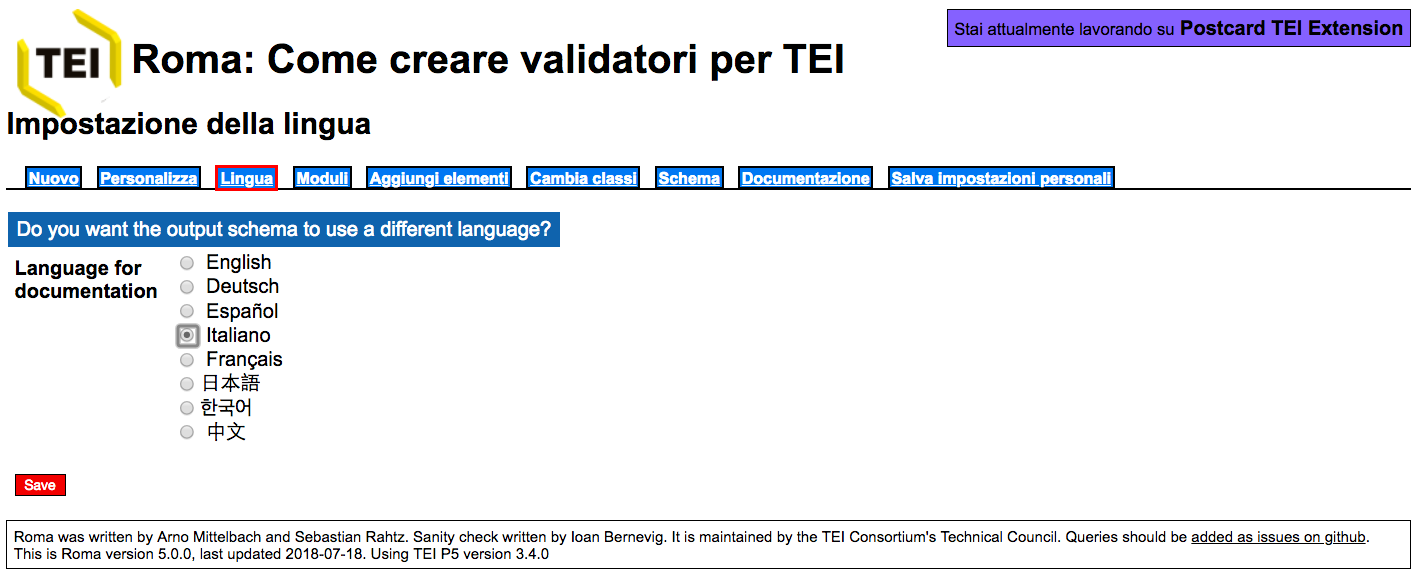
\includegraphics[width=.95\textwidth]{imgs/Roma3.png}
     \end{center}
   
    
\end{frame}

\begin{frame}
    \frametitle{Modulatirà e presonalizzazione della TEI}
    \addtocounter{nframe}{1}
    
    \textbf{Passo 3: Selezionare i moduli da includere}

     \begin{center}
        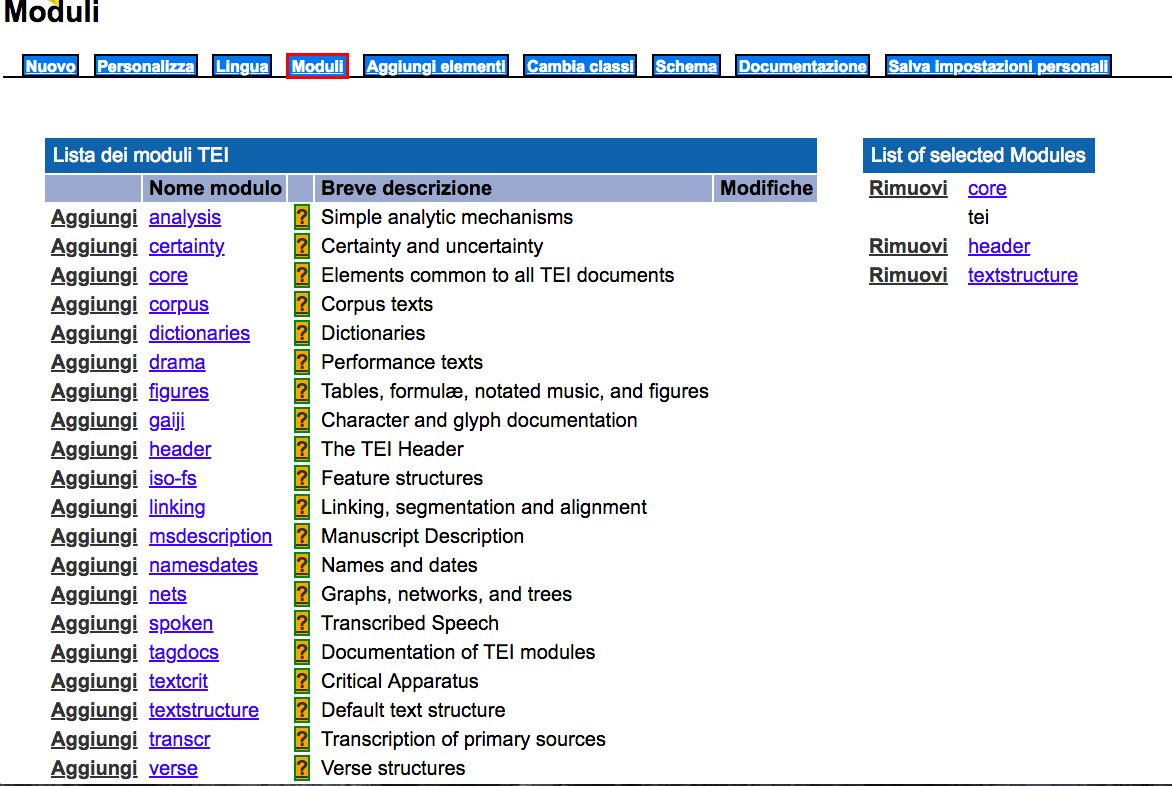
\includegraphics[width=.9\textwidth]{imgs/Roma4.png}
     \end{center}
   
    
\end{frame}

\begin{frame}
    \frametitle{Modulatirà e presonalizzazione della TEI}
    \addtocounter{nframe}{1}
    
    \textbf{Passo 4:  Rimuovere i moduli già inclusi}


     \begin{center}
        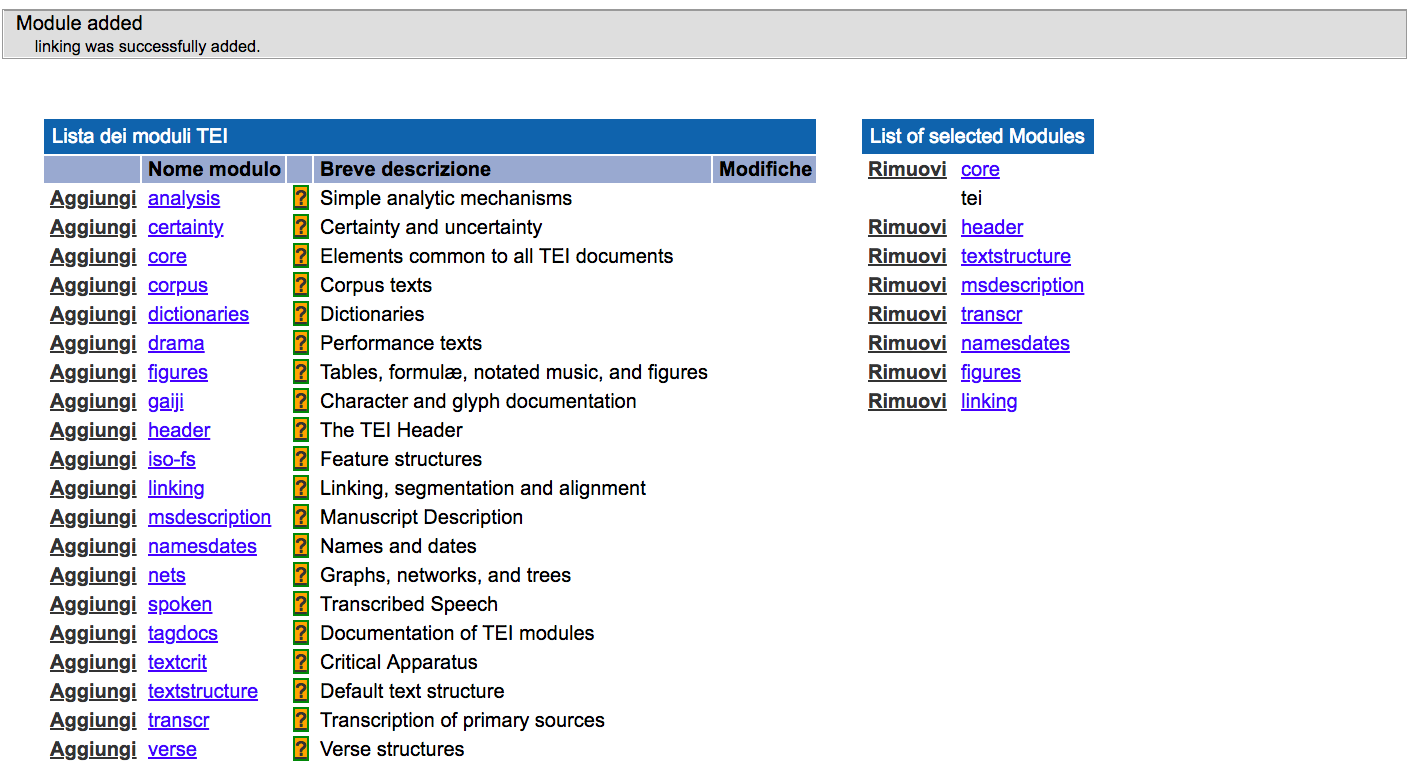
\includegraphics[width=.97\textwidth]{imgs/Roma5.png}
     \end{center}
   
    
\end{frame}

\begin{frame}
    \frametitle{Modulatirà e presonalizzazione della TEI}
    \addtocounter{nframe}{1}
    
    
    \textbf{Passo 5: Selezionare gli elementi da includere/escludere}

     \begin{center}
        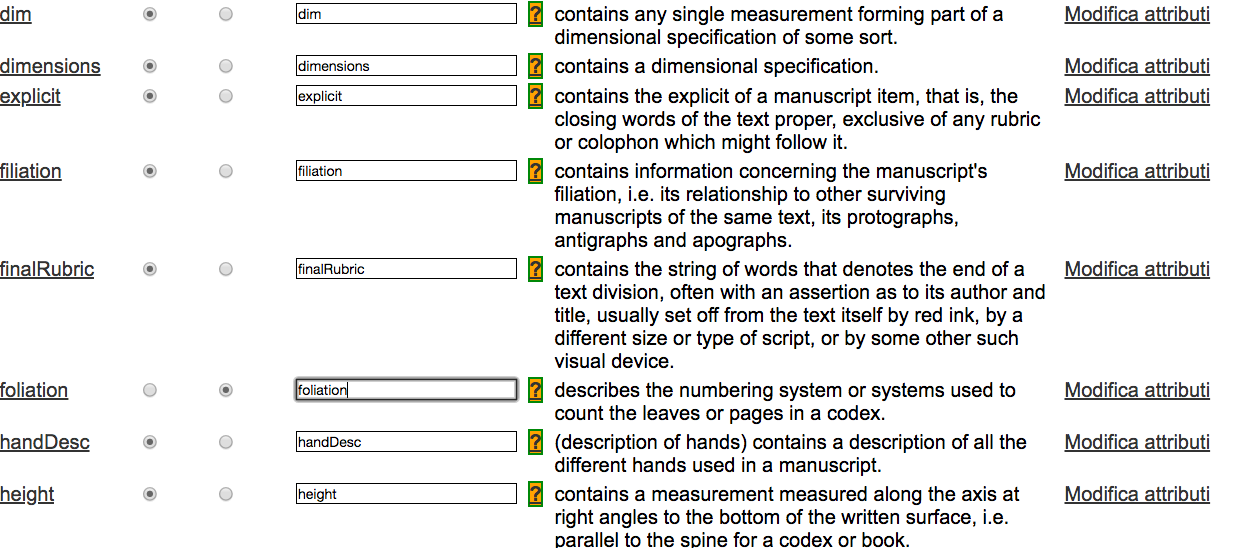
\includegraphics[width=.95\textwidth]{imgs/Roma6.png}
     \end{center}
   
    
\end{frame}

\begin{frame}
    \frametitle{Modulatirà e presonalizzazione della TEI}
    \addtocounter{nframe}{1}
    
    \textbf{Passo 6: Selezionare gli attributi da includere/escudere}

     \begin{center}
        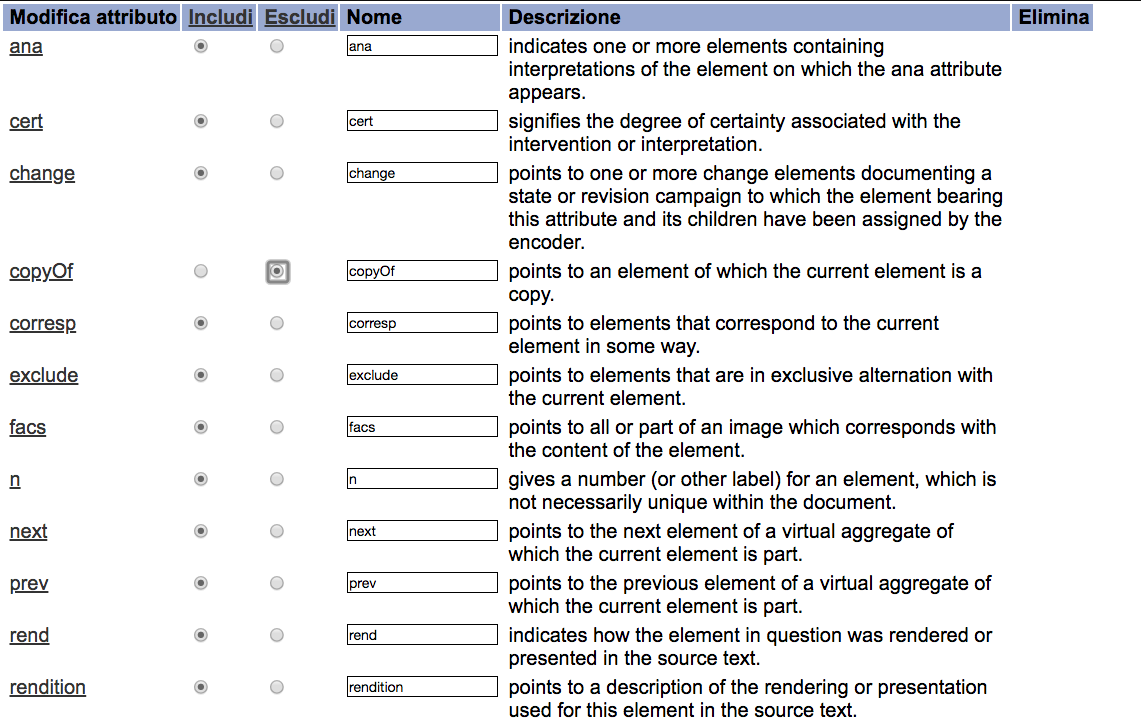
\includegraphics[width=.9\textwidth]{imgs/Roma7.png}
     \end{center}
   
    
\end{frame}

    
\begin{frame}
    \frametitle{Modulatirà e presonalizzazione della TEI}
    \addtocounter{nframe}{1}
    
    \textbf{Passo 7: Aggiungere uno o più nuovi elementi}

     \begin{center}
        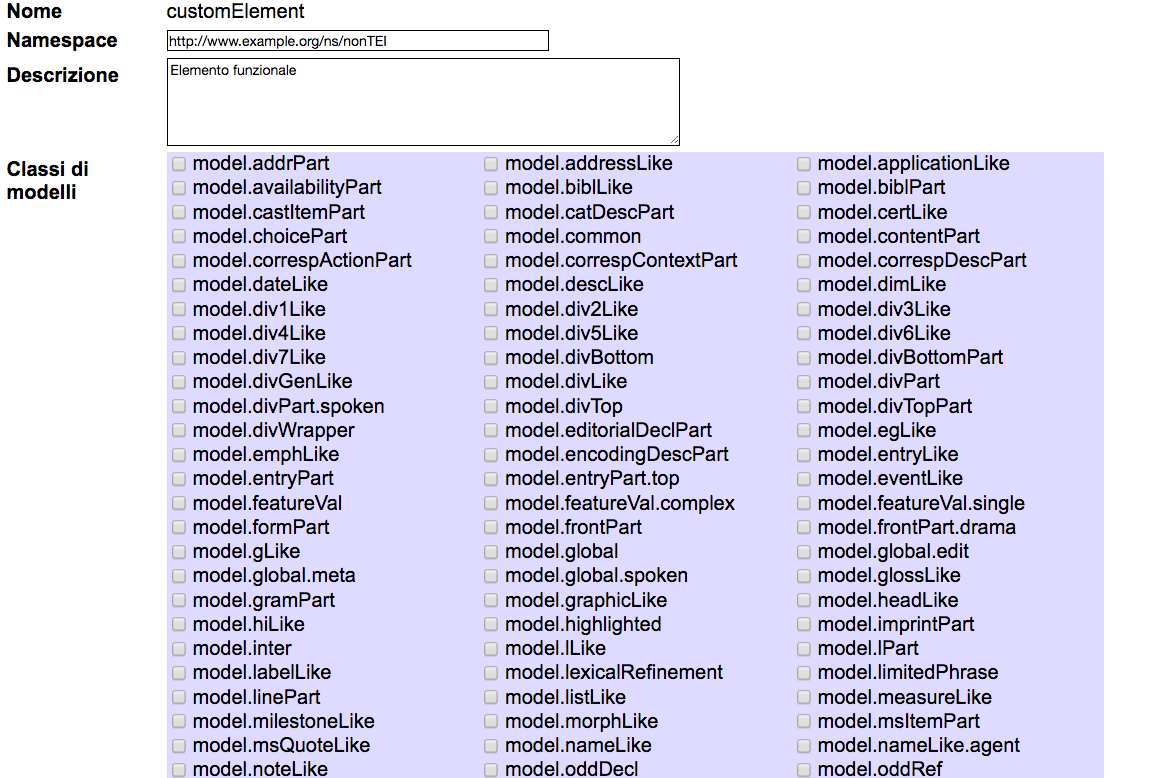
\includegraphics[width=.9\textwidth]{imgs/Roma9.png}
     \end{center}
    
\end{frame}
   
\begin{frame}
    \frametitle{Modulatirà e presonalizzazione della TEI}
    \addtocounter{nframe}{1}
    
    \textbf{Passo 8: Aggiungere uno o più nuovi attributi}

     \begin{center}
        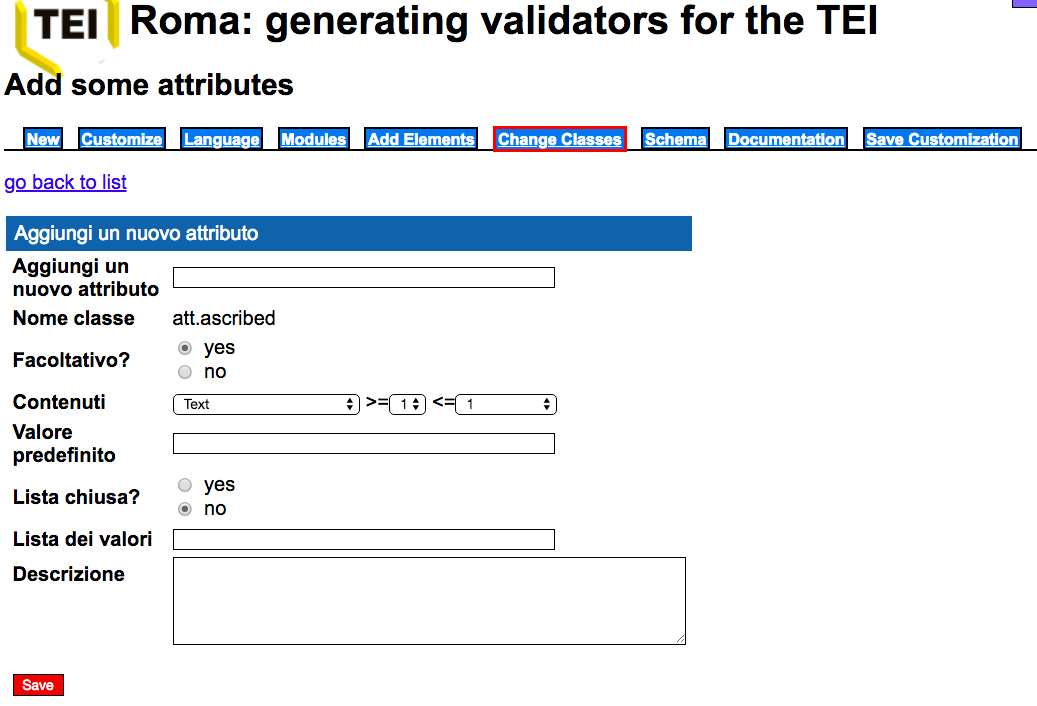
\includegraphics[width=.9\textwidth]{imgs/Roma14.png}
     \end{center}
     
    
\end{frame}
    
\begin{frame}
    \frametitle{Modulatirà e presonalizzazione della TEI}
    \addtocounter{nframe}{1}

    \textbf{Passo 9: Validare gli elementi e gli attributi inclusi}

     \begin{center}
        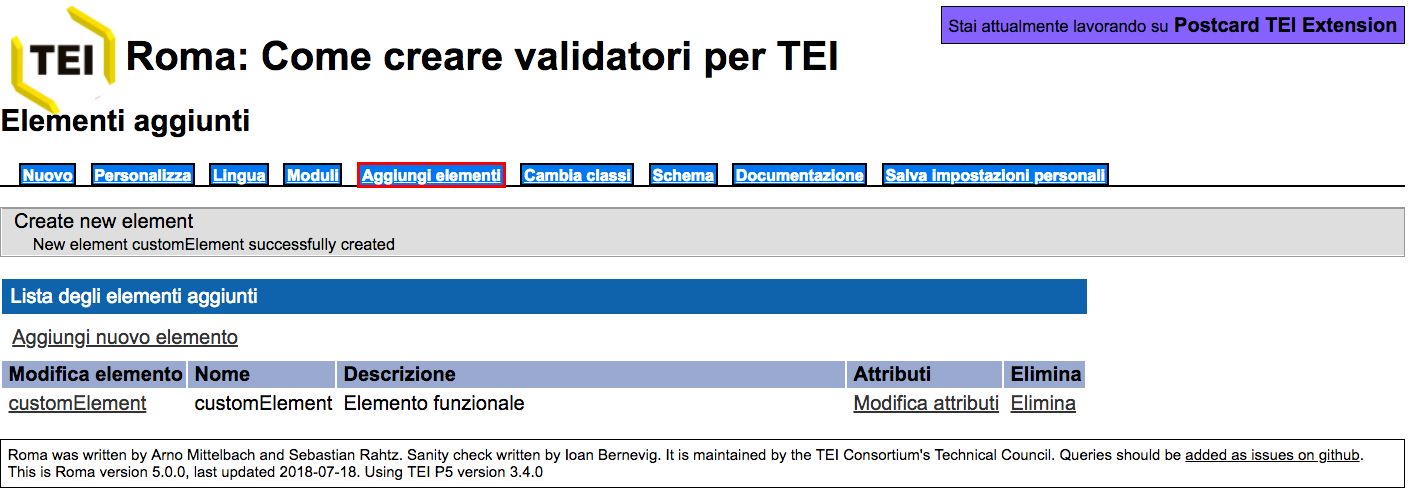
\includegraphics[width=.9\textwidth]{imgs/Roma8.png}
     \end{center}
   
    
\end{frame}


\begin{frame}
    \frametitle{Modulatirà e presonalizzazione della TEI}
    \addtocounter{nframe}{1}
    
    \textbf{Passo 10: personalizzare le classi predefinite TEI }

     \begin{center}
        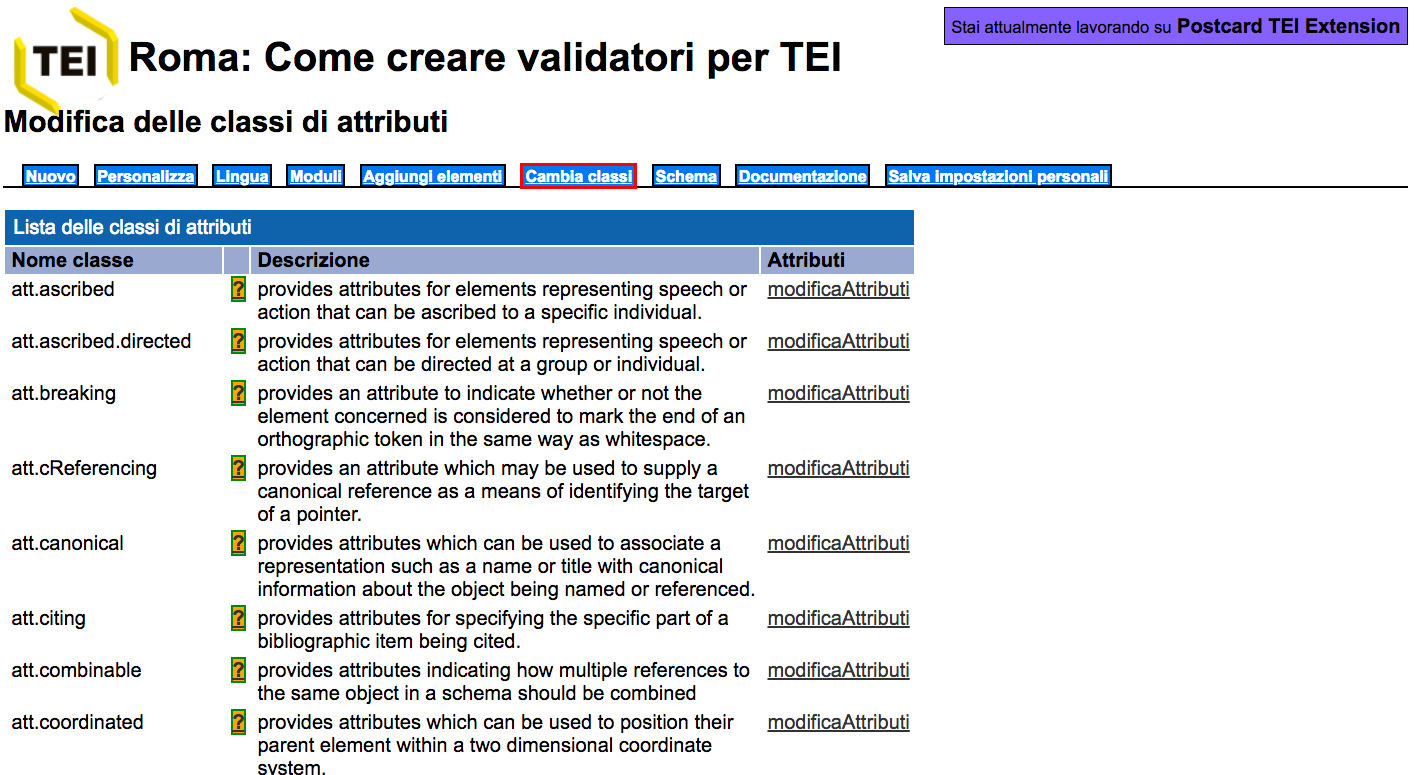
\includegraphics[width=.9\textwidth]{imgs/Roma10.png}
     \end{center}
   
    
\end{frame}

\begin{frame}
    \frametitle{Modulatirà e presonalizzazione della TEI}
    \addtocounter{nframe}{1}
    
    \textbf{Passo 11: Modificare le classi predefinite TEI}

     \begin{center}
        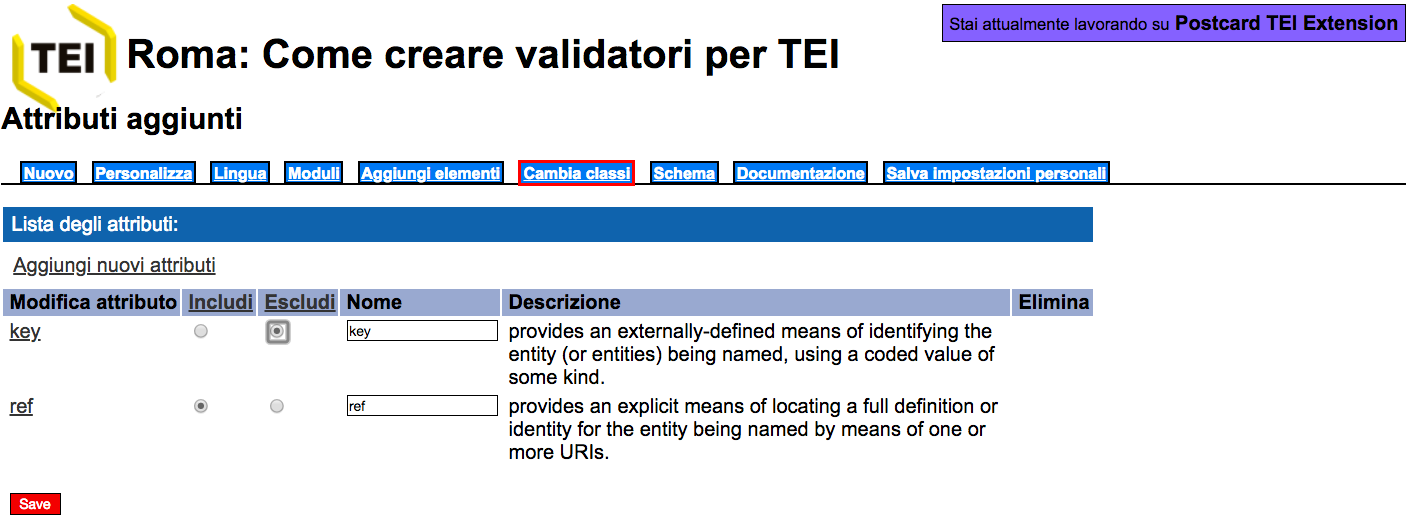
\includegraphics[width=.9\textwidth]{imgs/Roma11.png}
     \end{center}
   
    
\end{frame}

\begin{frame}
    \frametitle{Modulatirà e presonalizzazione della TEI}
    \addtocounter{nframe}{1}
   
   
    \textbf{Passo 12: Generazione dello schema}

     \begin{center}
        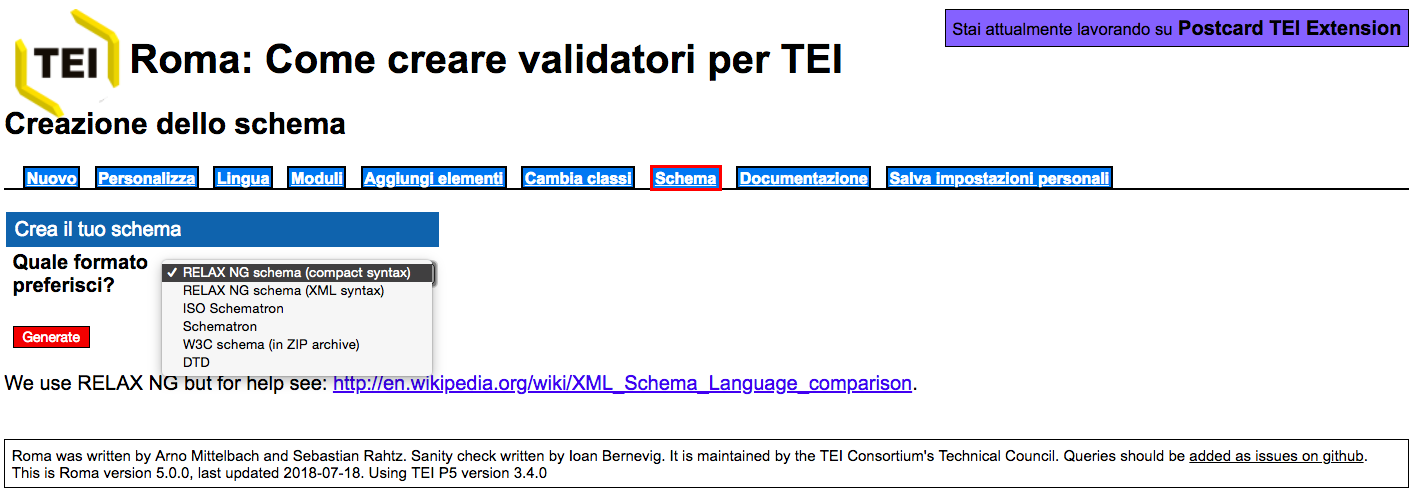
\includegraphics[width=.9\textwidth]{imgs/Roma12.png}
     \end{center}
   
    
\end{frame}

\begin{frame}
    \frametitle{Modulatirà e presonalizzazione della TEI}
    \addtocounter{nframe}{1}
    
    \textbf{Passo 13: Generazione della documentazione}

     \begin{center}
        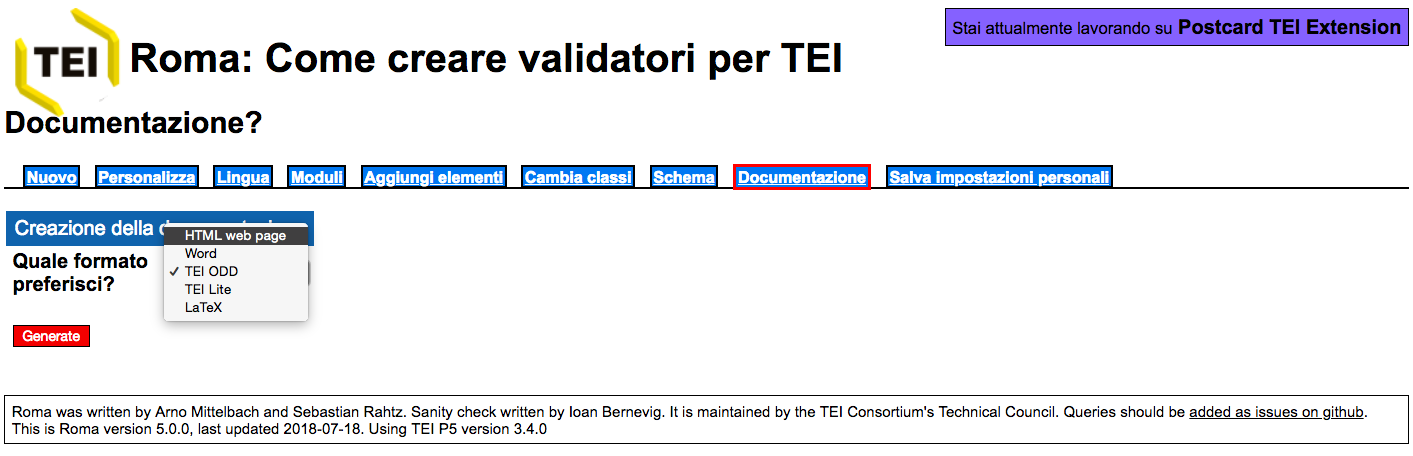
\includegraphics[width=.95\textwidth]{imgs/Roma13.png}
     \end{center}
    
\end{frame}

\begin{frame}
    \frametitle{Modulatirà e presonalizzazione della TEI}
    \addtocounter{nframe}{1}
    
    \textbf{Passo 14: Generazione del documento ODD}

     \begin{center}
        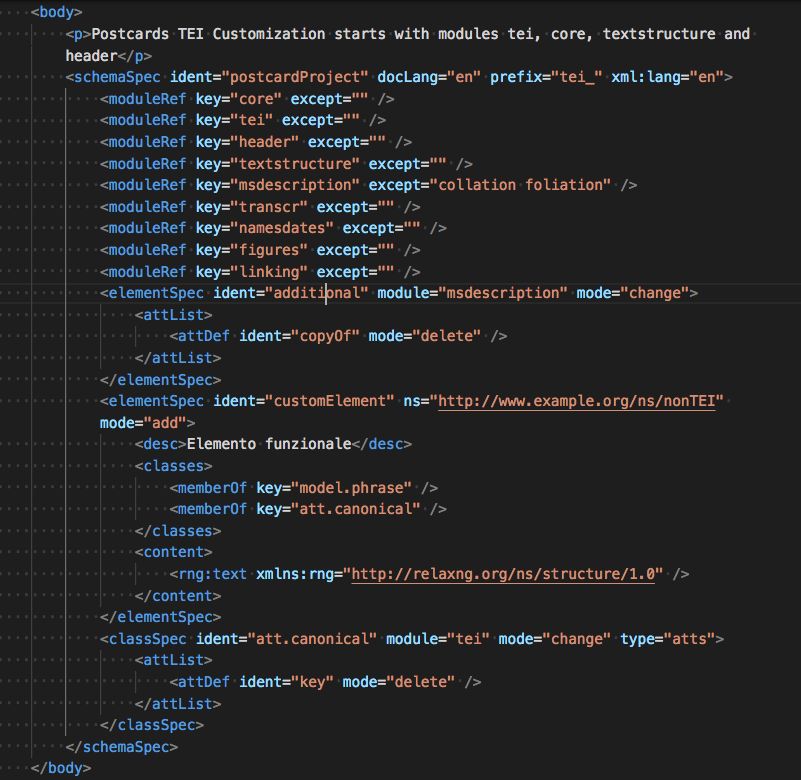
\includegraphics[width=.65\textwidth]{imgs/CustomizationODD.png}
     \end{center}
    
\end{frame}


\begin{frame}
    \frametitle{Modulatirà e presonalizzazione della TEI}
    \addtocounter{nframe}{1}
    
    \textbf{Documento ODD}

     \begin{center}
        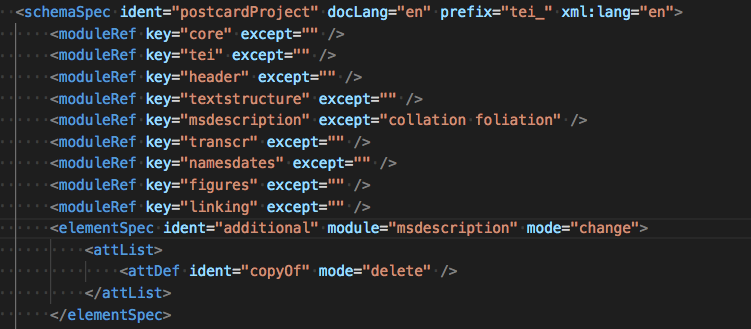
\includegraphics[width=.97\textwidth]{imgs/CustomizationODD-1.png}
     \end{center}
    
\end{frame}

\begin{frame}
    \frametitle{Modulatirà e presonalizzazione della TEI}
    \addtocounter{nframe}{1}
    
    \textbf{Documento ODD}

     \begin{center}
        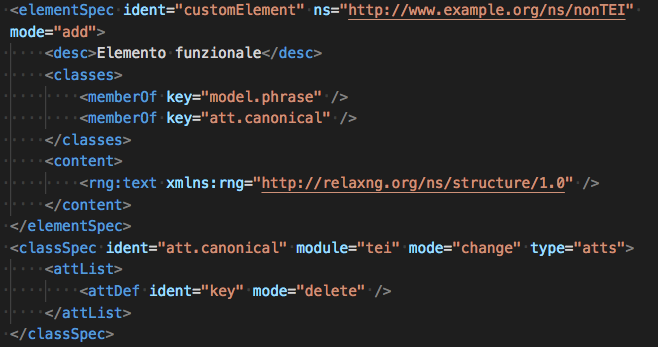
\includegraphics[width=.97\textwidth]{imgs/CustomizationODD-2.png}
     \end{center}
    
\end{frame}

\begin{frame}
    \frametitle{Modulatirà e presonalizzazione della TEI}
    \addtocounter{nframe}{1}
    
    \textbf{Schema dtd con le personalizzazioni}

     \begin{center}
        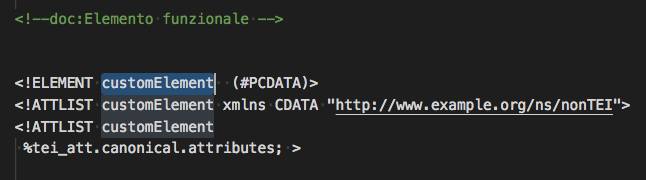
\includegraphics[width=.97\textwidth]{imgs/TEI-Custom-DTD.png}
     \end{center}
   
    
\end{frame}

\begin{frame}
    \frametitle{Modulatirà e presonalizzazione della TEI}
    \addtocounter{nframe}{1}
    
    \textbf{Schema dtd con le personalizzazioni}

     \begin{center}
        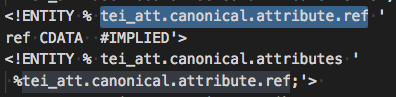
\includegraphics[width=.9\textwidth]{imgs/TEI-Custom-DTD-2.png}
     \end{center}
   
    
\end{frame}



\begin{frame}
    \frametitle{Modulatirà e presonalizzazione della TEI}
    \addtocounter{nframe}{1}

    \begin{block}{Approfondimenti}
            \begin{itemize}
                \item Customizing the TEI with Roma
                \item [] \url{http://www.tei-c.org/Guidelines/Customization/use_roma.xml}
                \item Getting Started with P5 ODDs
                \item [] \url{http://www.tei-c.org/Guidelines/Customization/odds.xml}
                \item TEI By Example: Customising TEI, ODD, Roma
                \item [] \url{http://teibyexample.org/modules/TBED08v00.htm}
            \end{itemize} 
    \end{block}

\end{frame}

    
    \section{Tematiche Avanzate per la codifica del testo in TEI}
    
    \begin{frame}
        \frametitle{Aspetti avanzati della TEI}
        \addtocounter{nframe}{1}
        
       % \begin{center}
        % 
\includegraphics[width=.2\textwidth]{../imgs/tei-r.pdf}
        % \end{center}
    
        \begin{itemize}
            
            \item<1-> Alcuni degli aspetti avanzati per la codifica TEI sono:
                \begin{itemize}
                    \item<1-> Gestione delle \textbf{Gerarchie Multiple Sovrapposte}
                    \item<1-> Annotazione e descrizione di \textbf{Entità Nominate}
                    \item<1-> Impiego dei \textbf{Namespace} per l'uso di più vocabolari XML
                    \item<1-> Impiego delle direttive \textbf{XInlude} per la gestione 
                     di documenti XML multipli
                \end{itemize} 
           
        \end{itemize}
        
    \end{frame}

    \begin{frame}
        \frametitle{Aspetti avanzati della TEI}
        \addtocounter{nframe}{1}
        
       % \begin{center}
        % 
\includegraphics[width=.2\textwidth]{../imgs/tei-r.pdf}
        % \end{center}
    
        \begin{block}{Modello Dati e Struttura XML: Singola Gerarchia}
            
            XML impone una singola gerarchia nel proprio modello dati che genera un singolo albero, dove non c’è alcuna possibilità di sovrapposizione.
           
        \end{block}
        
    \end{frame}


    \begin{frame}
        \frametitle{Aspetti avanzati della TEI}
        \addtocounter{nframe}{1}
        
       % \begin{center}
        % 
\includegraphics[width=.2\textwidth]{../imgs/tei-r.pdf}
        % \end{center}
    
        \begin{block}{Modello Dati e Struttura XML: Singola Gerarchia}
            
            Da un punto di vista della struttura e delle relazioni testuali che esistono implicitamente ed esplicitamente in una risorsa testuale, una singola gerarchia può non essere sufficiente a descrivere tutta la complessità veicolata. 
            
           
        \end{block}

        \begin{block}{Modello Dati e Struttura XML: Singola Gerarchia}

            E' necessario quindi considerare gerarchie multiple concorrenti per catturare contemporaneamente aspetti multipli e indipendenti (strutture sintattiche, dichiarazioni tipografiche, analisi semantiche o relazionali).

        \end{block}
        
    \end{frame}


    \begin{frame}
        \frametitle{Aspetti avanzati della TEI}
        \addtocounter{nframe}{1}
        
       % \begin{center}
        % 
\includegraphics[width=.2\textwidth]{../imgs/tei-r.pdf}
        % \end{center}
    
        \begin{block}{Gerarchie multiple sovrapposte}
            Uno stesso frammento di documento che si presta parzialmente o completamente ad essere annotato con tag differenti si può sovrapporre a gerarchie diverse dando vita a frammenti testuali che si intersecano gli uni agli altri.
        \end{block}

        \begin{block}{Gerarchie multiple sovrapposte: esempio}
            Per esempio un paragrafo può iniziare in una pagina e terminare all’interno della pagina successiva.
            \\ Per approfondire: \textit{TEI Guidelines 20 Non-hierarchical Structures}.
        \end{block}
        
    \end{frame}



    \begin{frame}
        \frametitle{Aspetti avanzati della TEI}
        \addtocounter{nframe}{1}
        
       % \begin{center}
        % 
\includegraphics[width=.2\textwidth]{../imgs/tei-r.pdf}
        % \end{center}
    \textit{Individuare gerarchie sovrapposte: codificare lo stesso testo con più prospettive.}

        \begin{block}{Esempio: Codifica della metrica}
            \begin{center}
                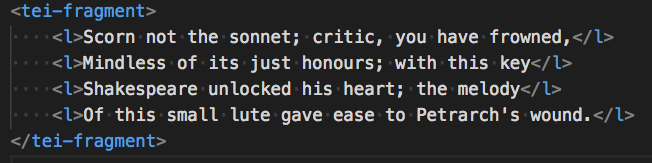
\includegraphics[width=.95\textwidth]{imgs/metrica.png}
            \end{center}
        \end{block}
        
    \end{frame}

    \begin{frame}
        \frametitle{Aspetti avanzati della TEI}
        \addtocounter{nframe}{1}
        
       % \begin{center}
        % 
\includegraphics[width=.2\textwidth]{../imgs/tei-r.pdf}
        % \end{center}
    \textit{Individuare gerarchie sovrapposte: codificare lo stesso testo con più prospettive.}

        \begin{block}{Esempio: Codifica delle frasi}
            \begin{center}
                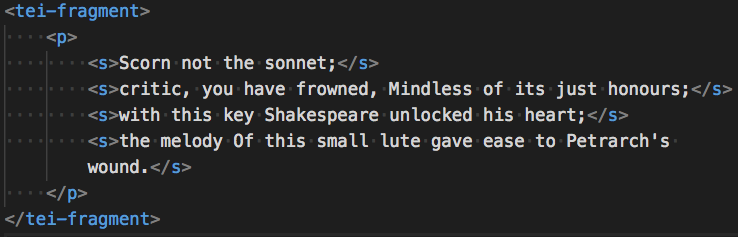
\includegraphics[width=.95\textwidth]{imgs/frasi.png}
            \end{center}
        \end{block}
        
    \end{frame}

    \begin{frame}
        \frametitle{Aspetti avanzati della TEI}
        \addtocounter{nframe}{1}
        
       % \begin{center}
        % 
\includegraphics[width=.2\textwidth]{../imgs/tei-r.pdf}
        % \end{center}

        \begin{block}{Gerarchie sovrapposte: Soluzioni proposte dalla TEI}
            \begin{itemize}
                \item Elementi vuoti
                \item Segmentazione
            \end{itemize}
        \end{block}
        
    \end{frame}


    \begin{frame}
        \frametitle{Aspetti avanzati della TEI}
        \addtocounter{nframe}{1}
        
       % \begin{center}
        % 
\includegraphics[width=.2\textwidth]{../imgs/tei-r.pdf}
        % \end{center}

        \begin{block}{Gerarchie sovrapposte: Elementi vuoti}
            Identificare un vocabolario come primario che viene rappresentato con una gerarchia standard XML, e usare elementi vuoti per delimitare l’inizio e la fine dei tag dei vocabolari secondari.
        \end{block}

        \begin{block}{Gerarchie sovrapposte: Elementi vuoti}
            Utilizzo di un elemento vuoto \textbf{milestone} che ha la funzione di marcare/segnare/annotare la posizione all’interno di un testo in cui la tipologia di un elemento in un dato sistema di riferimento cambia.
        \end{block}
        
    \end{frame}

    \begin{frame}
        \frametitle{Aspetti avanzati della TEI}
        \addtocounter{nframe}{1}
        
       % \begin{center}
        % 
\includegraphics[width=.2\textwidth]{../imgs/tei-r.pdf}
        % \end{center}
        Tali elementi non hanno contenuti, ma semplicemente suddividono il testo in regioni contigue
        \begin{block}{Gerarchie sovrapposte: Elementi vuoti}
            \begin{itemize}
                \item \texttt{<milestone/>}: segnala il limite che separa ogni tipo di sezione di un testo, come indicato da cambiamenti nel sistema di riferimento standard, qualora la sezione non sia rappresentata da un elemento strutturale.
                \item \texttt{<pb/>} (\textit{page beginning}): indica il limite tra una pagina di un testo e la successiva in un sistema di riferimento standard.
            \end{itemize}
        \end{block}

    \end{frame}

    \begin{frame}
        \frametitle{Aspetti avanzati della TEI}
        \addtocounter{nframe}{1}
        
       % \begin{center}
        % 
\includegraphics[width=.2\textwidth]{../imgs/tei-r.pdf}
        % \end{center}
        Tali elementi non hanno contenuti, ma semplicemente suddividono il testo in regioni contigue
        \begin{block}{Gerarchie sovrapposte: Elementi vuoti}
            \begin{itemize}
                \item \texttt{<lb/>} (\textit{line beginning}): segna l'inizio di una nuova riga (tipografica) in qualche edizione o versione di un testo.
                \item \texttt{<cb/>} (\textit{column beginning}): indica il limite tra una colonna di un testo e la successiva in un sistema di riferimento standard.
                \item \textbf{@n}: usato per codificare un valore per unità associate a milestone
            \end{itemize}
        \end{block}

    \end{frame}


    \begin{frame}
        \frametitle{Aspetti avanzati della TEI}
        \addtocounter{nframe}{1}
        
       % \begin{center}
        % 
\includegraphics[width=.2\textwidth]{../imgs/tei-r.pdf}
        % \end{center}
    \textit{Individuare gerarchie sovrapposte: codificare lo stesso testo con più prospettive.}

        \begin{block}{Esempio: Codificare righe e frasi}
            \begin{center}
                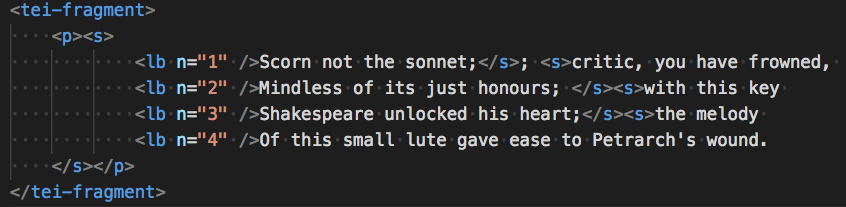
\includegraphics[width=.97\textwidth]{imgs/frasi-righe.png}
            \end{center}
        \end{block}
        
    \end{frame}

    \begin{frame}
        \frametitle{Aspetti avanzati della TEI}
        \addtocounter{nframe}{1}
        
       % \begin{center}
        % 
\includegraphics[width=.2\textwidth]{../imgs/tei-r.pdf}
        % \end{center}

        \begin{block}{Gerarchie sovrapposte: Segmentazione}
             Se un elemento appartenente ad una gerarchia secondaria è in overlap con elementi appartenenti alla gerarchia primaria, questo viene spezzato in frammenti più piccoli (\textbf{partial elements}).
        \end{block}

        \begin{block}{Gerarchie sovrapposte: Segmentazione}
            La gerarchia principale viene espressa attraverso markup XML standard, mentre gli elementi delle gerarchie secondarie risultano frammentati all'interno degli elementi principali: \textbf{sono connessi fra di loro attraverso attributi specifici}.
        \end{block}
        
    \end{frame}

    \begin{frame}
        \frametitle{Aspetti avanzati della TEI}
        \addtocounter{nframe}{1}
        
       % \begin{center}
        % 
\includegraphics[width=.2\textwidth]{../imgs/tei-r.pdf}
        % \end{center}

        \begin{block}{Gerarchie sovrapposte: Segmentazione}
              Modalità per collegare i \textbf{partial elements}.
              \begin{itemize}
                  \item \textbf{Virtual join}, chaining o aggregation
                  \item [] \textit{attraverso il meccanismo di co-indexing}
                  \item \textbf{Join}
                  \item [] \textit{attraverso collegamenti anche non contigui di elementi}
              \end{itemize}
        \end{block}

    \end{frame}

    \begin{frame}
        \frametitle{Aspetti avanzati della TEI}
        \addtocounter{nframe}{1}

        \begin{block}{Gerarchie sovrapposte: Co-indexing - Esempio}
            \begin{center}
                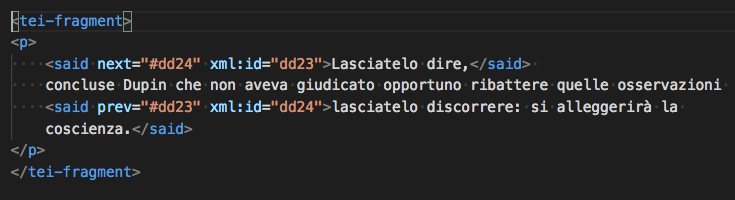
\includegraphics[width=.97\textwidth]{imgs/co-indexing.png}
            \end{center}
        \end{block}

            \tiny\textit{Lasciatelo dire, – concluse Dupin che non aveva giudicato opportuno ribattere quelle osservazioni – lasciatelo discorrere: si alleggerirà la coscienza.}

    \end{frame}

    \begin{frame}
        \frametitle{Aspetti avanzati della TEI}
        \addtocounter{nframe}{1}

        \begin{block}{Gerarchie sovrapposte: Join - Esempio}
            \begin{center}
                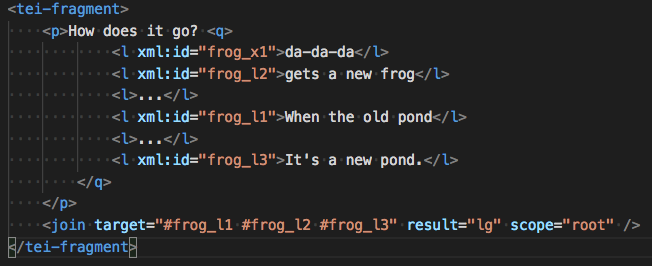
\includegraphics[width=.95\textwidth]{imgs/join.png}
            \end{center}
        \end{block}
    \end{frame}

    \begin{frame}
        \frametitle{Aspetti avanzati della TEI}
        \addtocounter{nframe}{1}

        \begin{block}{Entità Nominate: definizione poco rigorosa}
            Sono definite \textbf{entità nominate} (\textit{named entities}) quegli ``oggetti'' del \textit{mondo reale} (\textbf{persone}, \textbf{luoghi}, \textbf{organizzazioni}, ecc.) che possono essere designati ed individuati in maniera precisa per mezzo di \textbf{nomi propri}.
        \end{block}
    \end{frame}

    \begin{frame}
        \frametitle{Aspetti avanzati della TEI}
        \addtocounter{nframe}{1}

        \begin{block}{Entità Nominate e TEI}
            In un testo possiamo trovare molti riferimenti a oggetti nominati.
            \\In TEI possono essere codificati in vario modo.
        \end{block}
        
            \begin{itemize}
                \item \texttt{<rs>}
                \item \texttt{<name>}
                \item \texttt{<persName>}
                \item \texttt{<placeName>}
                \item ...
            \end{itemize}
        
    \end{frame}

    \begin{frame}
        \frametitle{Aspetti avanzati della TEI}
        \addtocounter{nframe}{1}

        \begin{block}{Entità Nominate e TEI}
            Un nome da solo, tuttavia, presenta sempre margini di ambiguità che impediscono una identificazione univoca sulla base del testo.
        \end{block}

        \begin{block}{Entità Nominate e TEI}
            Per questo motivo si raccolgono gli oggetti nominati, individuati nel testo, in liste specifiche.
            \\ Le singole occorrenze dei nomi condificate nel testo si collegano poi a queste liste per mezzo di opportuni riferimenti. 
        \end{block}
        
    \end{frame}

    \begin{frame}
        \frametitle{Aspetti avanzati della TEI}
        \addtocounter{nframe}{1}
        
        \textit{Nel \texttt{<teiHeader>} sarà inserita una lista dedicata alle persone}

            \begin{center}
                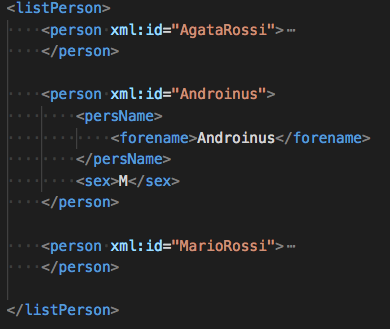
\includegraphics[width=.7\textwidth]{imgs/listPerson.png}
            \end{center}
        
    \end{frame}

    \begin{frame}
        \frametitle{Aspetti avanzati della TEI}
        \addtocounter{nframe}{1}

        \begin{block}{Entità nominate: Name - Esempio}
            \begin{center}
                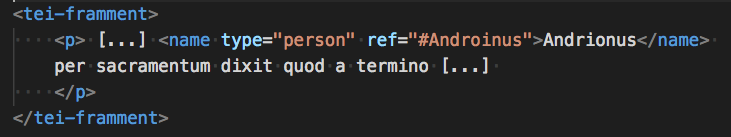
\includegraphics[width=.98\textwidth]{imgs/name.png}
            \end{center}
        \end{block}
        \textit{Nel testo si riferisce la persona in questione attraverso l'attributo \textbf{@ref} che identifichi un \textbf{@xml:id} specifico per la persona marcata}
    \end{frame}

    \begin{frame}
        \frametitle{Aspetti avanzati della TEI}
        \addtocounter{nframe}{1}

        \begin{block}{Entità nominate}
            \begin{itemize}
                \item Qualunque forma ortografica e lessicale riconducibile alla stessa persona avrà un puntatore allo stesso valore di \textbf{@xml:id}
                \item Volendo può essere applicato anche a \textbf{forme denotative} meno precise e/o allusive: \textit{il Presidente degli Stati Uniti}.
            \end{itemize}
        \end{block}
    \end{frame}

    \begin{frame}
        \frametitle{Aspetti avanzati della TEI}
        \addtocounter{nframe}{1}

        \begin{block}{Entità nominate: Luoghi, Enti, Organizzazioni, ecc}
            \begin{itemize}
                \item Lo stesso metodo si applica anche ai nomi di luogo
                \item [] Utilizzando l'elemento \texttt{<listPlace>}
                \item Lo stesso metodo si applica anche ai nomi di enti e organizzazioni
                \item [] Utilizzando l'elemento \texttt{<listOrg>}
            \end{itemize}
        \end{block}
    \end{frame}


    \begin{frame}
        \frametitle{Aspetti avanzati della TEI}
        \addtocounter{nframe}{1}

        \begin{block}{NameSpace}
            \begin{itemize}
                \item i \textbf{namespace} sono dei raggruppamenti di nomi sotto un unico identificativo
                \item possibilità di usare gli elementi di più vocabolari contemporaneamente
                \item distinguere gli elementi di ciascun vocabolario
                \item indicare lo schema di appartenenza per gli elementi
                \item distinguere elementi e attributi con lo stesso nome
            \end{itemize}
        \end{block}
    \end{frame}


    \begin{frame}
        \frametitle{Aspetti avanzati della TEI}
        \addtocounter{nframe}{1}

        \begin{block}{Uso dei NameSpace}
            \begin{itemize}
                \item i \textbf{namespace} sono dei raggruppamenti di nomi sotto un unico identificativo
                \item per introdurre un namespace nel documento XML si utilizza l'attributo \textbf{@xmlns}.
                \item il valore dell'attributo \textbf{@xmlns} è un \textbf{URI} che non ha nessun valore dichiarativo, ma solo \textbf{informativo}.
                \item \texttt{<elemento xmlns="URI" />}
                \item \texttt{<prefix:elemento xmlns:prefix="URI" />}
            \end{itemize}
        \end{block}
    \end{frame}

    \begin{frame}
        \frametitle{Aspetti avanzati della TEI}
        \addtocounter{nframe}{1}

        
            \begin{center}
                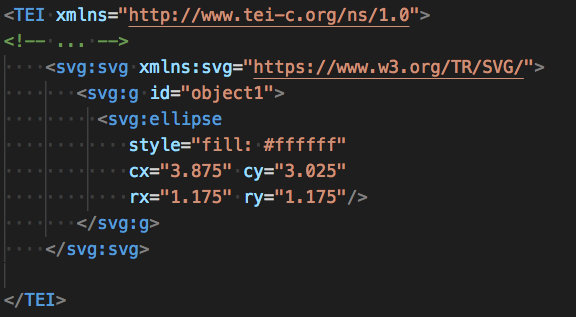
\includegraphics[width=.9\textwidth]{imgs/namespaces.png}
            \end{center}
        \textit{Ogni nome di elemento o attributo del documento XML è preceduto da un prefisso che specifica il vocabolario di appartenenza}
    \end{frame}

    \begin{frame}
        \frametitle{Aspetti avanzati della TEI}
        \addtocounter{nframe}{1}

        \begin{block}{XInclude}
            XInclude (XML Inclusions) è una sintassi e un modello di elaborazione che specifica un metodo generale di inclusione di oggetti all’interno dei documenti XML.
        \end{block}
        \textit{Pagina W3C della tecnologia: \url{https://www.w3.org/TR/xinclude/}}
    \end{frame}

    \begin{frame}
        \frametitle{Aspetti avanzati della TEI}
        \addtocounter{nframe}{1}

        \begin{block}{XInclude: possibilità}
            \begin{itemize}
                \item si possono inserire all’interno di documenti XML altri documenti, in parte o in toto
                \item molto utile nel caso si abbia a che fare con documenti multipli che condividono caratteristiche comuni, ad esempio i testi di un manoscritto o un corpus
            \end{itemize}
        \end{block}
    \end{frame}


    \begin{frame}
        \frametitle{Aspetti avanzati della TEI}
        \addtocounter{nframe}{1}

        \begin{block}{XInclude: sintassi di base}
            \begin{itemize}
                \item Elementi e Namespace
                \item [] \texttt{<xi:include xmlns:xi="http://www.w3.org/2001/XInclude" />}
                \item [] \texttt{<xi:fallback>}: copre le risorse mancanti
                \item Attributi
                \item [] \texttt{@xpointer}: identifica parte della risorsa da includere; se omesso viene inclusa tutta la risorsa
                \item [] \texttt{@href}: URI che specifica la posizione della risorsa
            \end{itemize}
        \end{block}
        
    \end{frame}

    \begin{frame}
        \frametitle{Aspetti avanzati della TEI}
        \addtocounter{nframe}{1}
        
            \begin{center}
                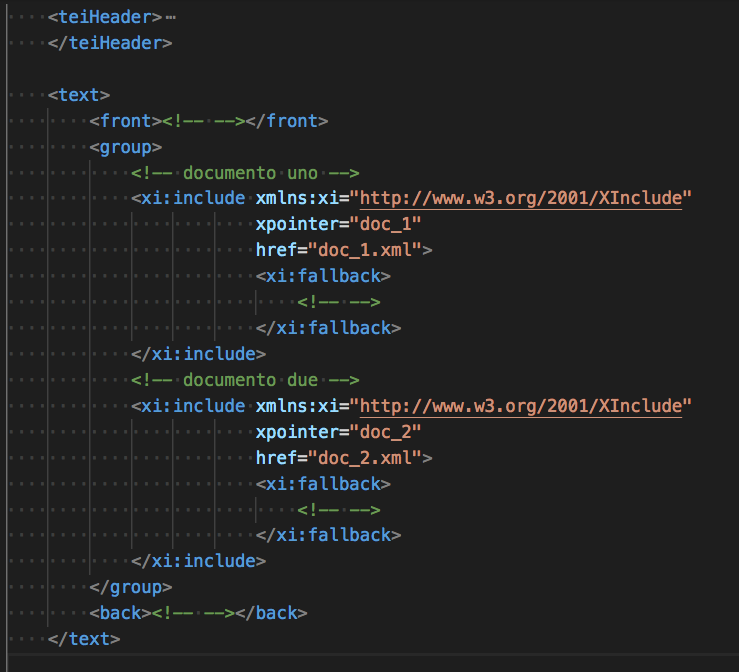
\includegraphics[width=.8\textwidth]{imgs/xinclude.png}
            \end{center}
        
    \end{frame}
    \begin{frame}
        \frametitle{Aspetti avanzati della TEI}
        \addtocounter{nframe}{1}
        
            \begin{center}
                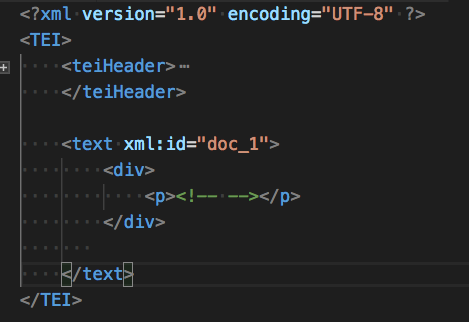
\includegraphics[width=.95\textwidth]{imgs/doc_1.png}
            \end{center}
        
    \end{frame}
    \begin{frame}
        \frametitle{Aspetti avanzati della TEI}
        \addtocounter{nframe}{1}
        
            \begin{center}
                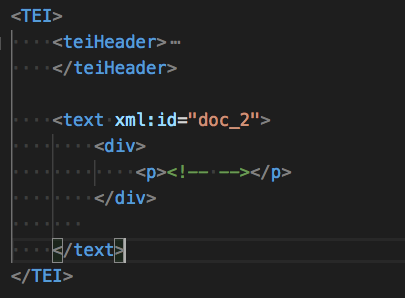
\includegraphics[width=.85\textwidth]{imgs/doc_2.png}
            \end{center}
        
    \end{frame}


    
    \section{Conclusioni}
    % strumenti per la pubblicazione
% strumenti per l'analisi (TXM, altri)
% slides James Cummings 
% customizzazione TEI vedere capitoli 22 e 23 delle guidelines
    
    \end{document}